\documentclass{article}
\usepackage{cmap}
\usepackage[utf8]{inputenc}
\usepackage[english,ukrainian]{babel}
\usepackage{graphicx}
\usepackage{geometry}
\usepackage{listings}
\usepackage{float}
\usepackage{amsmath}
\geometry{
	a4paper,
	left=20mm,
	right=20mm,
	top=15mm,
	bottom=15mm,
}
\lstset{
	language=c,
	tabsize=4,
	keepspaces,
	showstringspaces=false,
}
\graphicspath{ {./pictures} }
\setlength{\parindent}{4em}

\newcommand\subject{Організація комп’ютерних мереж}
\newcommand\lecturer{асистент кафедри ПЗ \\ Задорожний І.М.}
\newcommand\teacher{асистент кафедри ПЗ \\ Задорожний І.М.}
\newcommand\mygroup{ПЗ-22}
\newcommand\lab{2}
\newcommand\theme{Дослідження роботи протоколів ІР та ICMP}
\newcommand\purpose{Ознайомитися з принципами роботи та призначенням протоколів IP та ICMP
	та за допомогою утиліт ping, tracert та аналізатора протоколів Wireshark ознайомитися зі
	структурою пакетів цих протоколів}

\begin{document}
\begin{normalsize}
	\begin{titlepage}
		\thispagestyle{empty}
		\begin{center}
			\textbf{МІНІСТЕРСТВО ОСВІТИ І НАУКИ УКРАЇНИ\\
				НАЦІОНАЛЬНИЙ УНІВЕРСИТЕТ "ЛЬВІВСЬКА ПОЛІТЕХНІКА"}
		\end{center}
		\begin{flushright}
			\textbf{ІКНІ}\\
			Кафедра \textbf{ПЗ}
		\end{flushright}
		\vspace{200pt}
		\begin{center}
			\textbf{ЗВІТ}\\
			\vspace{10pt}
			до лабораторної роботи № \lab\\
			\textbf{на тему}: “\textit{\theme}”\\
			\textbf{з дисципліни}: “\subject”
		\end{center}
		\vspace{112pt}
		\begin{flushright}
			
			\textbf{Лектор}:\\
			\lecturer\\
			\vspace{28pt}
			\textbf{Виконав}:\\
			
			студент групи \mygroup\\
			Коваленко Д.М.\\
			\vspace{28pt}
			\textbf{Прийняв}:\\
			
			\teacher\\
			
			\vspace{28pt}
			«\rule{1cm}{0.15mm}» \rule{1.5cm}{0.15mm} 2023 р.\\
			$\sum$ = \rule{1cm}{0.15mm}……………\\
			
		\end{flushright}
		\vspace{\fill}
		\begin{center}
			\textbf{Львів — 2023}
		\end{center}
	\end{titlepage}
		
	\begin{description}
		\item[Тема.] \theme.
		\item[Мета.] \purpose.
	\end{description}

\section*{Теоретичні відомості}
\begin{enumerate}
	\item[7.] Які параметри є в команди ping? - ping [-t] [-a] [-n число] [-l число] [-f] [-i TTL] [-v TOS] [-r число] [-s число] [[-j
	списоквузлів | [-k списоквузлів]] [-w таймаут] КінцевеІм’я
	Параметри:\\
	-t Відправлення до переривання.\\
	-n Число запитів.\\
	-l Розмір відправлення.\\
	-f Встановлення прапорця DF.\\
	-w Час очікування.
	\item[8.] Які параметри має команда tracert? - tracert [-d] [-h макс число] [-j список вузлів] [-w інтервал] ім'я
	Параметри:\\
	-d Без визначення адрес по іменах вузлів.\\
	-h макс число Максимальне число переходів при пошуку вузла.\\
	-j список вузлів Вільний вибір маршруту за списком вузлів.\\
	-w інтервал Інтервал чекання кожної відповіді в мілісекундах
	\item[20.] Що трапляється з пакетами, в яких контрольна сума неправильна?
	Вони відкидаються.
\end{enumerate}

\section*{Хід виконання}
\begin{figure}[H]
	\centering
	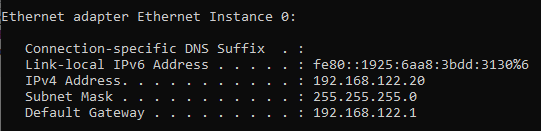
\includegraphics[scale=0.8]{ic}
	\caption{Виконання утиліти ipconfig}
\end{figure}

\begin{figure}[H]
	\centering
	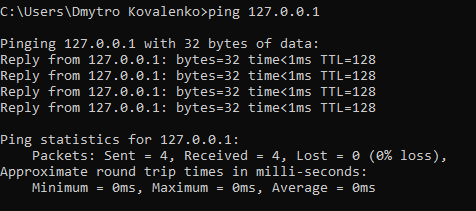
\includegraphics[scale=0.8]{pl}
	\caption{Замикання на себе}
\end{figure}

\begin{figure}[H]
	\centering
	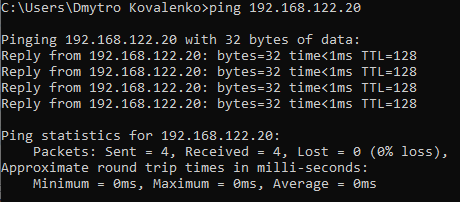
\includegraphics[scale=0.8]{p12220}
	\caption{Відгук власного комп'ютера}
\end{figure}

\begin{figure}[H]
	\centering
	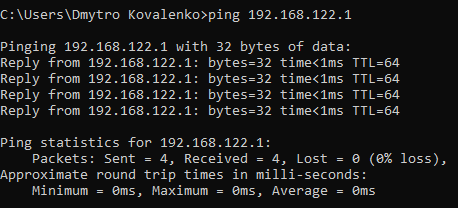
\includegraphics[scale=0.8]{p1221}
	\caption{Відгук шлюзу}
\end{figure}

\begin{figure}[H]
	\centering
	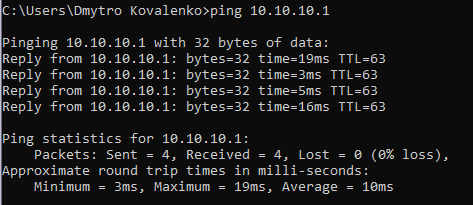
\includegraphics[scale=0.8]{p101}
	\caption{Відгук віддаленого вузла}
\end{figure}

\begin{figure}[H]
	\centering
	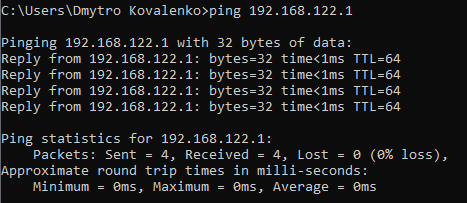
\includegraphics[scale=0.8]{pdns}
	\caption{Відгук DNS сервера}
\end{figure}

\begin{figure}[H]
	\centering
	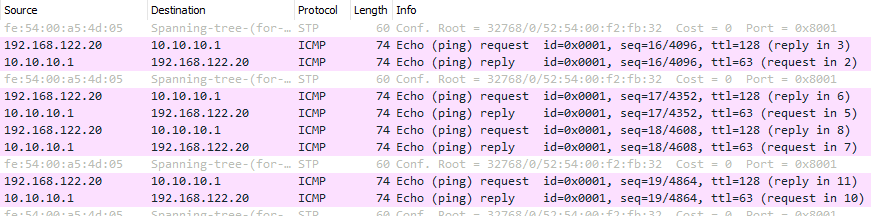
\includegraphics[scale=0.55]{prw}
	\caption{Перехоплені пакети під час виконання команди ping до віддаленого вузла}
\end{figure}

\begin{figure}[H]
	\centering
	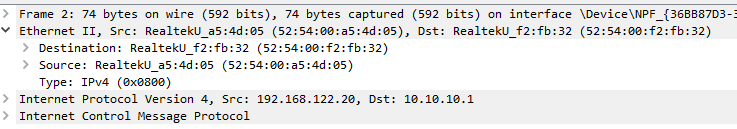
\includegraphics[scale=0.65]{prw2}
	\caption{Будова перехоплених пакетів під час виконання команди ping до віддаленого вузла}
\end{figure}

З рис.8 видно, що власна MAC адреса - 52:54:00:a5:d4:05, а MAC адреса віддаленого вузла - 52:54:00:f2:fb:32

\begin{figure}[H]
	\centering
	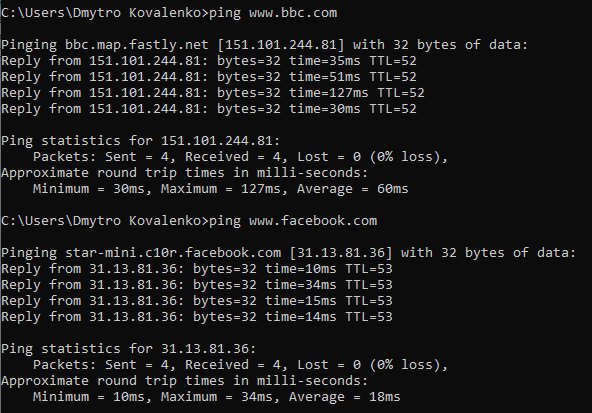
\includegraphics[scale=0.8]{bbcfacebook}
	\caption{Відправлення ехо-запитів на віддалені вузли відповідно до варіанту}
\end{figure}

\begin{figure}[H]
	\centering
	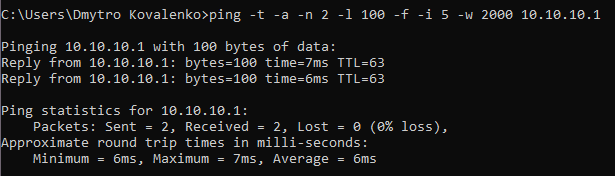
\includegraphics[scale=0.8]{pall}
	\caption{Випробування усіх параметрів команди ping}
\end{figure}

\begin{figure}[H]
	\centering
	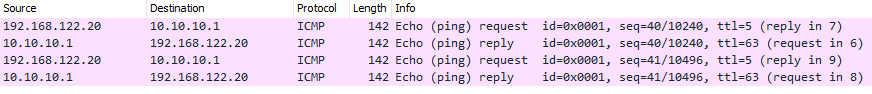
\includegraphics[scale=0.55]{2}
	\caption{Перехоплені пакети під час випробування усіх параметрів команди ping}
\end{figure}

\begin{figure}[H]
	\centering
	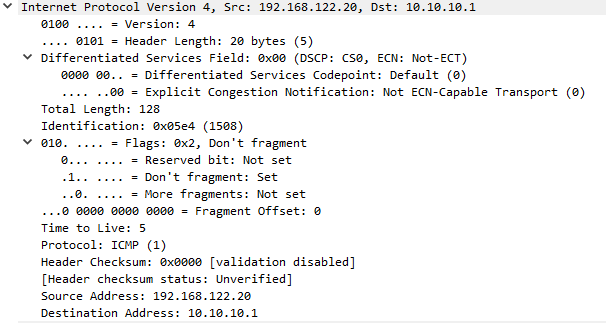
\includegraphics[scale=0.8]{22}
	\caption{Вміст перехоплених пакетів під час випробування усіх параметрів команди ping}
\end{figure}

\begin{figure}[H]
	\centering
	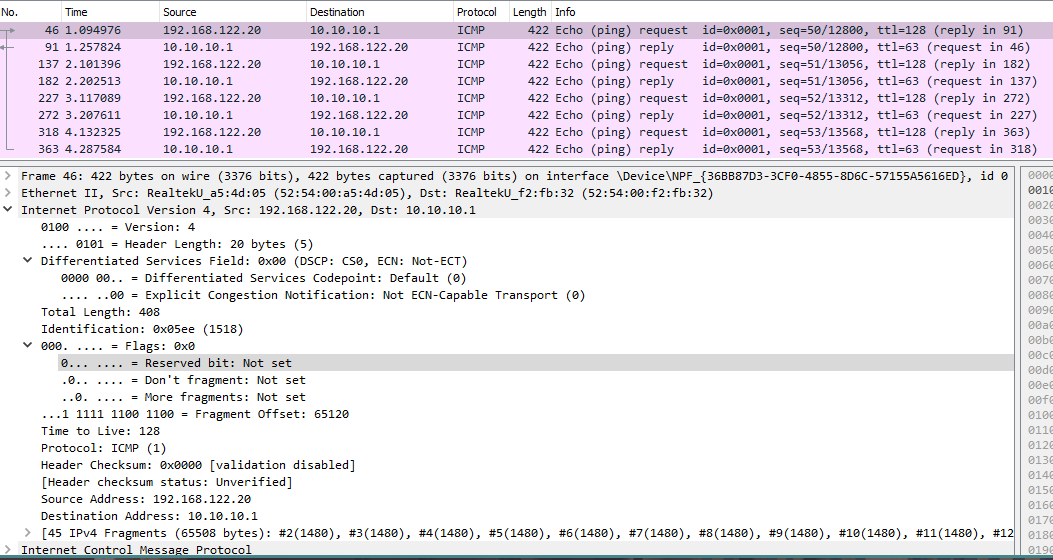
\includegraphics[scale=0.45]{l}
	\caption{Дослідження фрагментації з прапорцем -l}
\end{figure}

\begin{figure}[H]
	\centering
	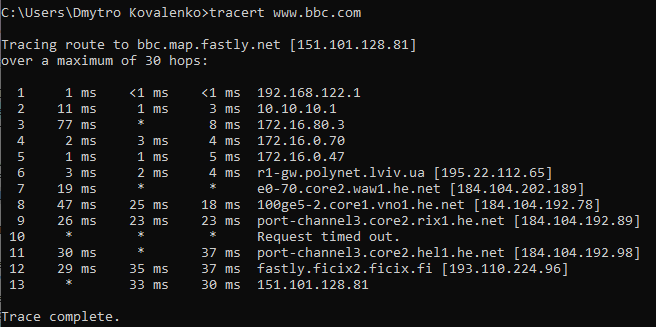
\includegraphics[scale=0.65]{t1}
	\caption{Трасування маршруту за допомогою утиліти tracert}
\end{figure}

\begin{figure}[H]
	\centering
	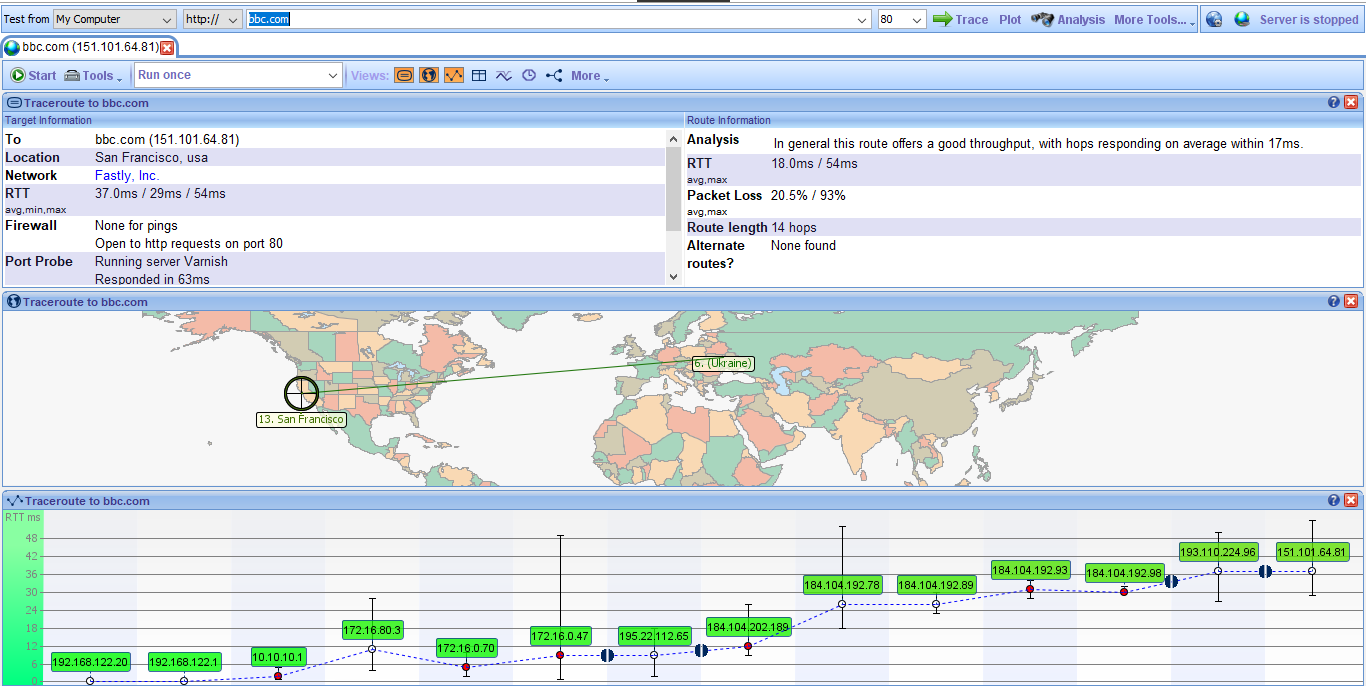
\includegraphics[scale=0.35]{t2}
	\caption{Трасування маршруту за допомогою утиліти VisualRoute}
\end{figure}

\begin{figure}[H]
	\centering
	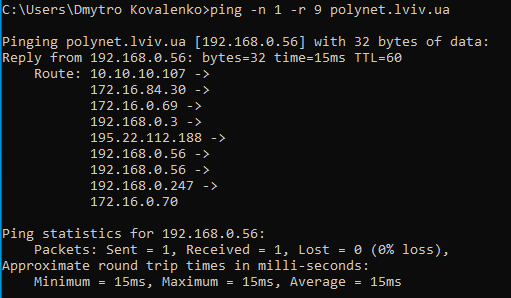
\includegraphics[scale=0.8]{3}
	\caption{Трасування маршруту за допомогою утиліти ping з параметром -r}
\end{figure}

Яким чином обчислюється контрольна сума? Наведіть приклади.
В інтернет-протоколі контрольна сума обчислюється для забезпечення цілісності даних, які передаються між різними вузлами мережі.

Контрольна сума обчислюється на основі заголовку та корисних даних пакету IP. Заголовок пакету містить інформацію про джерело та призначення пакету, а також інші параметри. Для обчислення контрольної суми використовуються алгоритми хешування, які перетворюють дані на контрольну суму фіксованої довжини.

\section*{Висновки}
Під час виконання лабораторної роботи я ознайомився з принципами роботи та призначенням протоколів IP та ICMP та за допомогою утиліт ping, tracert та аналізатора протоколів Wireshark ознайомився зі структурою пакетів цих протоколів.
	    
\end{normalsize}
\end{document}
